

\title{\LARGE \bf
Dimentionless Policies based on the Buckingham $\pi$ Theorem: \\ 
Is it a good way to Generalize Numerical Results?
}


%\author{Alexandre~Girard,~\IEEEmembership{Member,~IEEE,}
%        and~H.~Harry~Asada,~\IEEEmembership{Member,~IEEE}% <-this % stops a space
\author{Alexandre Girard$^{1}$% <-this % stops a space
\thanks{$^{1}$Alexandre Girard is with the Department of Mechanical Engineering, Universite de Sherbrooke, Qc, Canada {\tt\small  alex.girard@usherbrooke.ca }}% <-this % stops a space
}%


% make the title area
\maketitle
\thispagestyle{empty}
\pagestyle{empty}


\begin{abstract}
Yes if the context are dimentionnaly similar. Here we show that by modifying the problem formulation of the pendulum swing-up task using dimentionless variables, we can re-use the optimal policy generated numerically for any pendulum that are dimentionnaly similar. We also demonstrate that by leveraging this scheme when using reinforcement learning, multiple systems of various dimentions can share a data-base during the learning phase, which can be a big advantage for data efficiency. It remains to be seen if this approach can also help generalizing policies for more complex high-dimentional problems.
\end{abstract}

%%%%%%%%%%%%%%%%%%%%%%
\section{Introduction}

Many numerical algorithms = black box mapping

System and problem parameters are not explicitly in the function




%%%%%%%%%%%%%%%%%%%%%%%%%%%%%%%%%%%%%%%%%%%%
\subsection{Context variables in the policy mapping}

For a specific system, a control policy takes the form of mapping from a vector space $x$ representing the state $x$ of the dynamic system to be controlled, and a vector space representing the control inputs $u$ of the system. 
%%%%%%%%%%%%%%%%%%%%%%
\begin{equation}
u
=
f \left(
x
\right)
\end{equation}
%%%%%%%%%%%%%%%%%%%%%%
Under some assumptions (mainly a fully observable systems and an infinite time horizon), the optimal policy is also guarantee to be of this form [Cite Bertsekas]

To consider the question of how can this policy or knowledge can be transfer in a different context, it is usefull to think about a higher dimension mapping, that we will note $\pi$, also having arguments a vector of variables $c$ describing the context:
%%%%%%%%%%%%%%%%%%%%%%
\begin{equation}
u
=
\pi \left(
x,
c
\right)
\end{equation}
%%%%%%%%%%%%%%%%%%%%%%



%%%%%%%%%%%%%%%%%%%%%%
\begin{figure}[H]
\vspace{-5pt}
\begin{center}
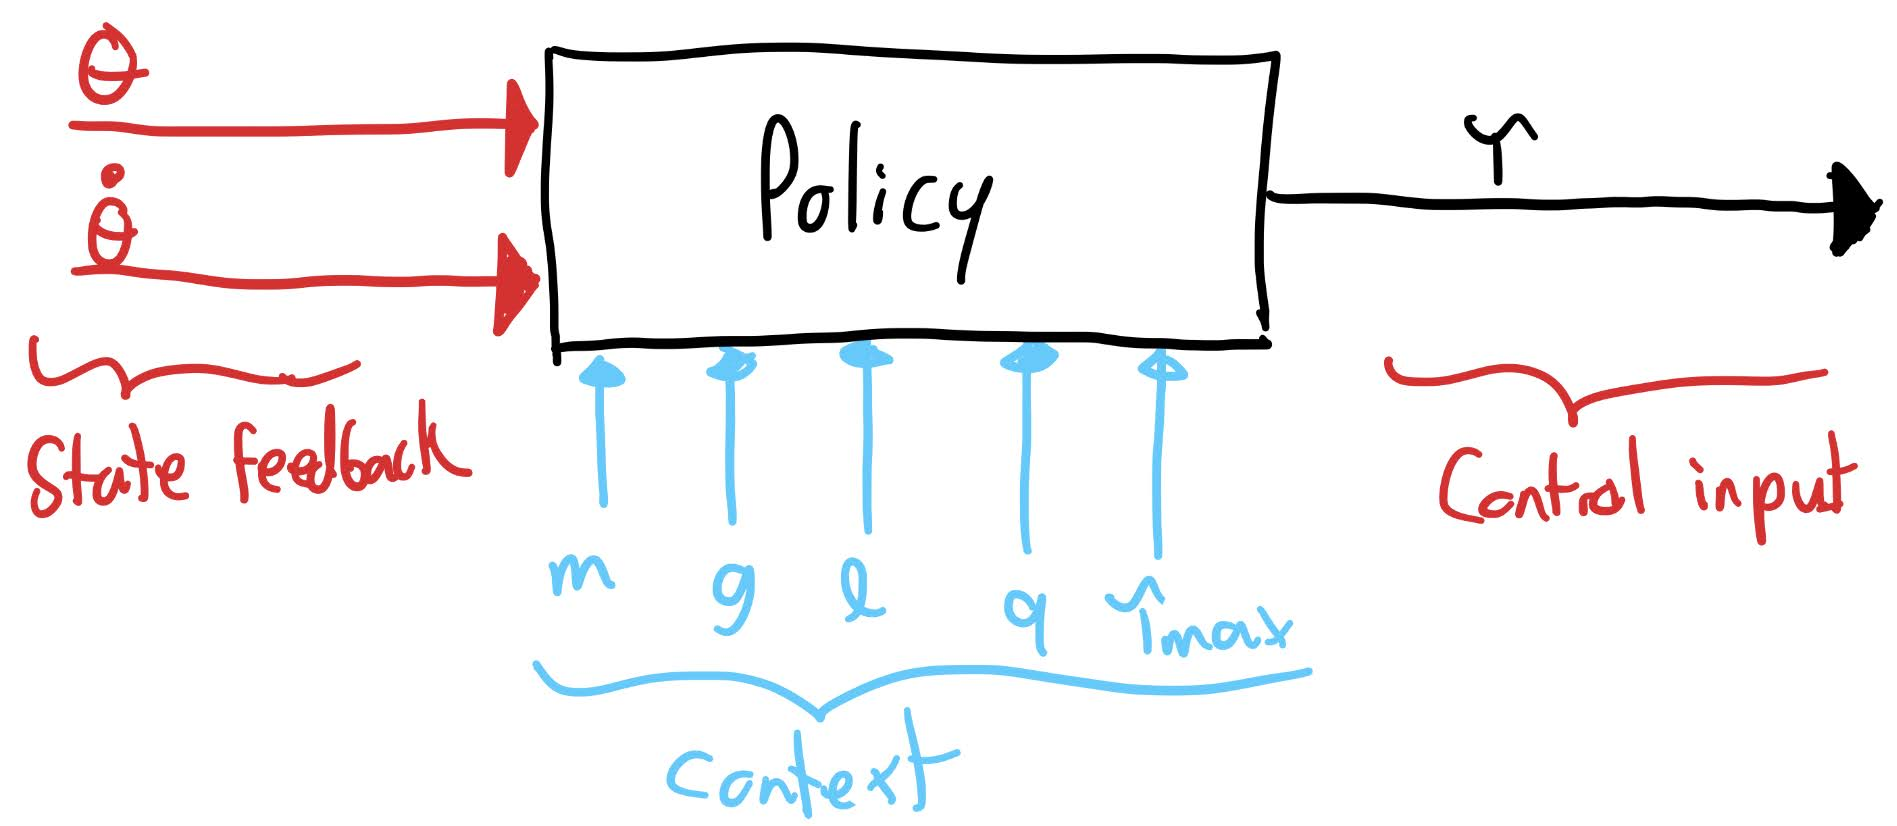
\includegraphics[width=0.75\linewidth]{fig/policy_context.jpg}
\caption{For the pendulum swing-up task, the context is 5 variables: the parameter of the system: $m$, $g$, and $l$, a parameter of the cost function: $q$ and a parameter defining the constraints: $\tau_{max}$.
}\label{fig:policy_context}
\end{center}
\vspace{-5pt}
\end{figure}
%%%%%%%%%%%%%%%%%%%%%%

%%%%%%%%%%%%%%%%%%%%%%
\begin{figure}[t]
\vspace{-5pt}
\begin{center}
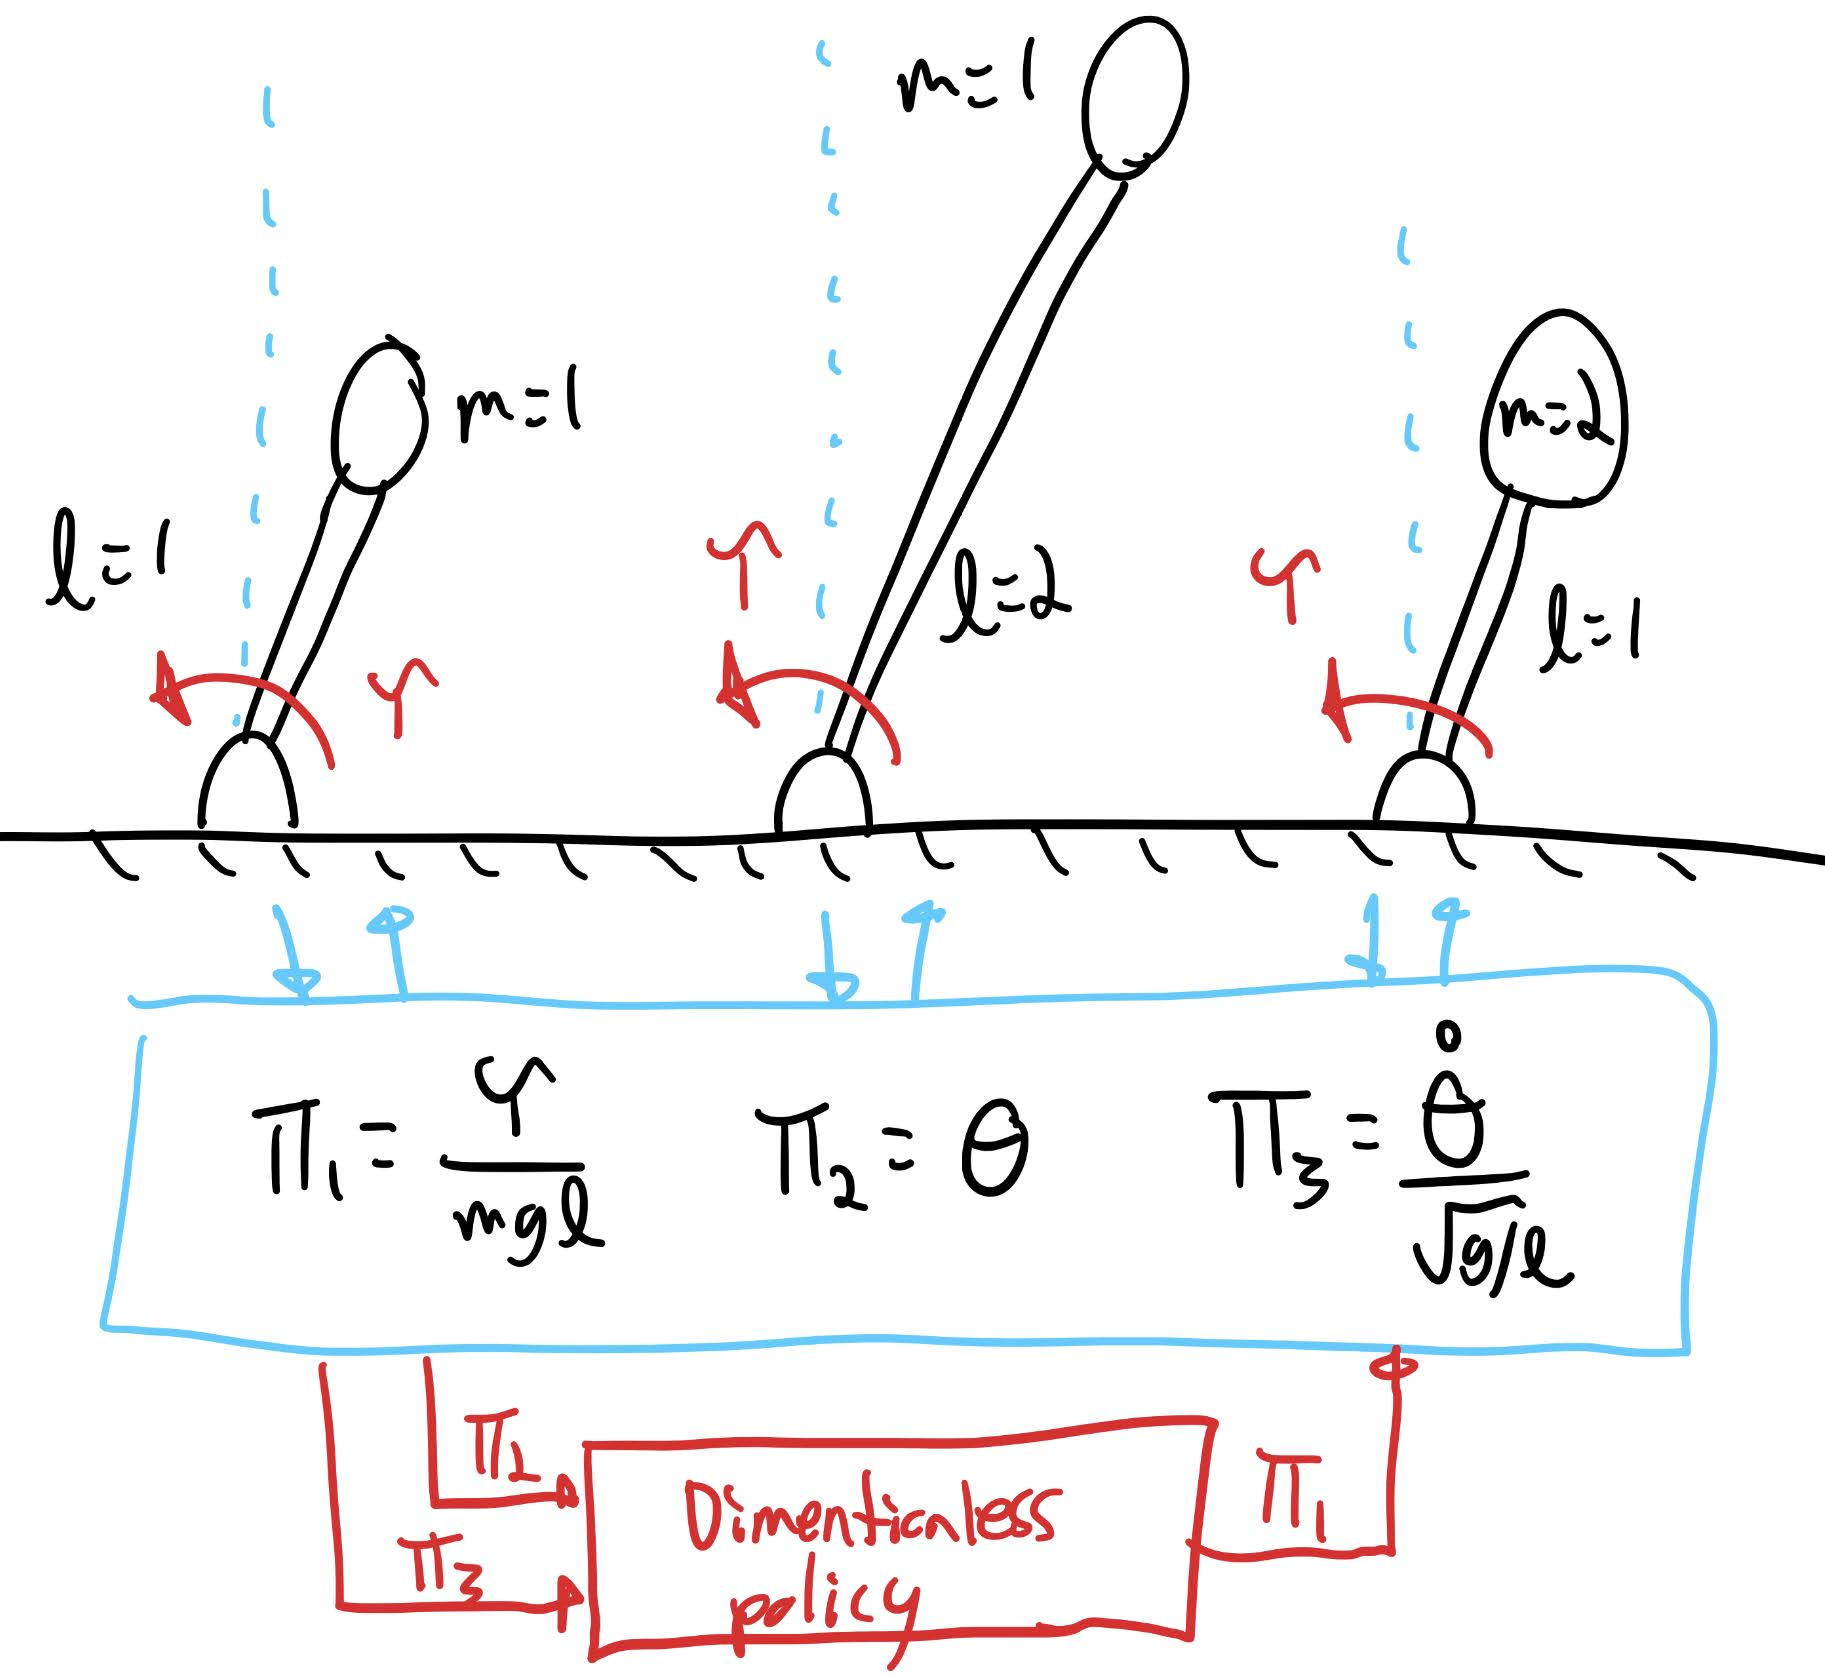
\includegraphics[width=0.99\linewidth]{fig/big_picture.jpg}
\caption{Big picture}\label{fig:big_picture}
\end{center}
\vspace{-15pt}
\end{figure}
%%%%%%%%%%%%%%%%%%%%%%

The context must include all the variables, system parameters and task parameters, that would affect the  policy:
%%%%%%%%%%%%%%%%%%%%%%
\begin{equation}
\underbrace{\begin{bmatrix}
u_1 \\
\vdots \\
u_k
\end{bmatrix}}_{\text{inputs}}
=
\pi \left(
\underbrace{\begin{bmatrix}
x_1 \\
\vdots \\
x_n
\end{bmatrix}}_{\text{states}}
,
\underbrace{
\underbrace{\begin{bmatrix}
a_1 \\
\vdots \\
\vdots \\
a_m
\end{bmatrix}}_{\text{system}}
,
\underbrace{\begin{bmatrix}
b_1 \\
\vdots \\
b_l
\end{bmatrix}}_{\text{task}}
}_{\text{Context $c$}}
\right) 
\label{eq:vectorpolicy}
\end{equation}
%%%%%%%%%%%%%%%%%%%%%%

Then we can formalize the goal of generalizing a policy to a different context: if a good feedback policy $f_1$ is found for a system in a context described by variables $c_1$, can this knowledge help finding an equivalent good feedback policy in a different context $c_2$?
%%%%%%%%%%%%%%%%%%%%%%
\begin{equation}
\pi \left(
x,
c = c_1
\right) = 
f_1 \left(
x 
\right) 
\quad \Rightarrow \quad
\pi \left(
x,
c = c_2
\right) = ?
\end{equation}
%%%%%%%%%%%%%%%%%%%%%%
Using the Buckinham Pi theorem [Cite something], we will show that if a dimentionless version of the context is equal, then a dimentionless version of the policy mapping must be also equivalent.


% %%%%%%%%%%%%%%%%%%%%%%
% \begin{figure}[H]
% \begin{center}
% 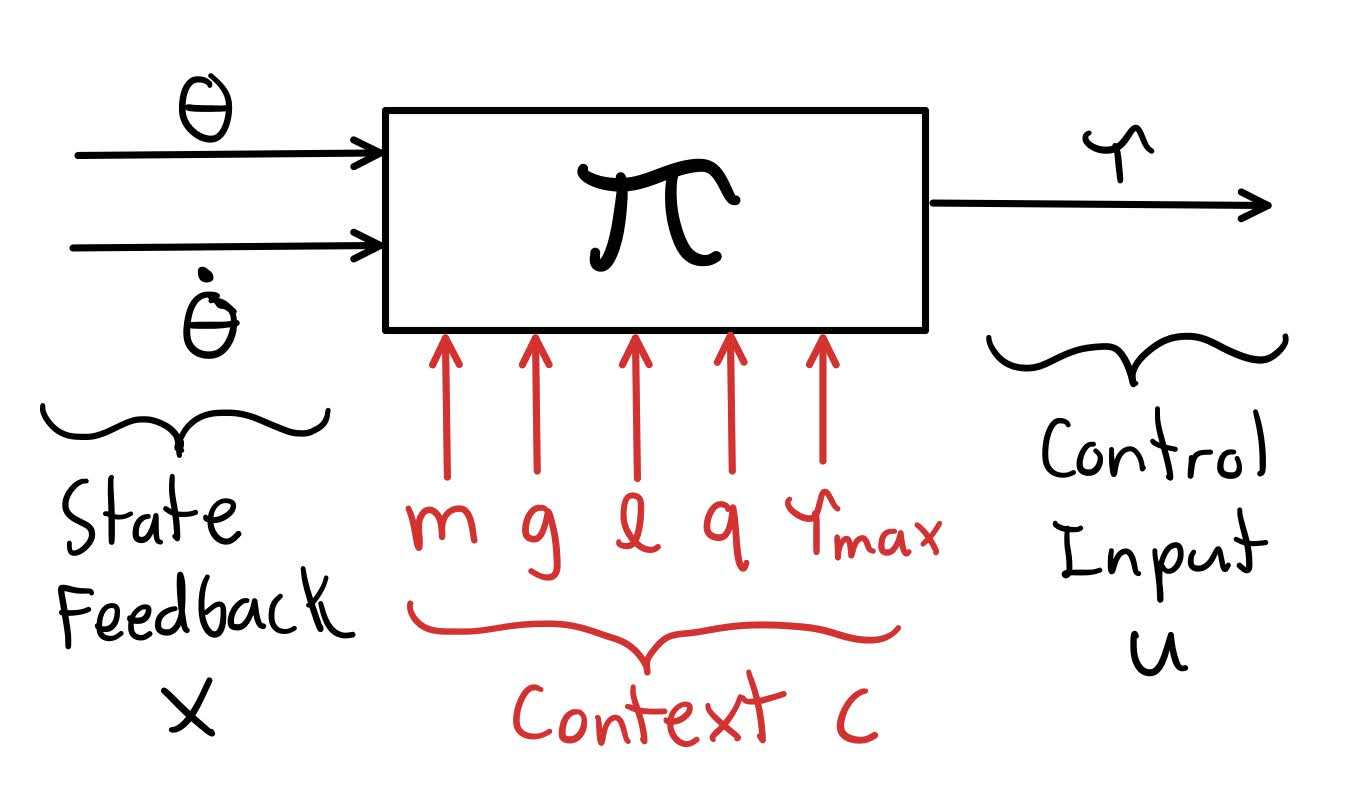
\includegraphics[width=0.99\linewidth]{fig/policy_context2.jpg}
% \caption{Big picture}\label{fig:policy_context}
% \end{center}
% \end{figure}
% %%%%%%%%%%%%%%%%%%%%%%

\subsection{Dimentional analysis of the augmented policy mapping}

If the policy involve $k$ control input variables, then we can treat the augmented policy as $k$ mapping from states and context variables to the scalar control input $j$:
%%%%%%%%%%%%%%%%%%%%%%
\begin{equation}
u_j = \pi_j \left(
x_1, \hdots, x_n, 
a_1, \hdots \hdots, a_m, 
b_1, \hdots, b_l, 
\right) 
\label{eq:scalarpolicy}
\end{equation}
%%%%%%%%%%%%%%%%%%%%%%
% %%%%%%%%%%%%%%%%%%%%%%
% \begin{equation}
% u_j = \pi_j \left(
% x,
% c 
% \right) \quad j = \{ 1, \hdots , k \}
% \end{equation}
% %%%%%%%%%%%%%%%%%%%%%%
where eq. \eqref{eq:scalarpolicy} is the $j$th line of the policy in vector form described by eq. \eqref{eq:vectorpolicy}.
Then, if the state vector is define by $n$ variables, and the context is defined by $m$ system parameters plus $l$ tasks parameters, then each mapping $\pi_j$ involves $1 + n + m + l$ (usually dimentionnal) variables. Dimentional analysis is based on the fact that those mapping describe a function that should not fundenmentaly depends on the system of units involved, this is formalized with Buckingham Pi theorem. Applying the Buckingham Pi theorem to this relashionship, tell us that if $d$ dimensions are involved in all thoses variables, then an equivalent dimentionless relationship between $p$ dimentionless $\Pi$ groups, where:
%%%%%%%%%%%%%%%%%%%%%%
\begin{equation}
p \geq (1 + n + m + l ) - d
\end{equation}
%%%%%%%%%%%%%%%%%%%%%%
Assuming $d$ dimentions are involved in the $m$ system parameter, and that we are in a situation where the maximum reduction is possinle $p = (1 + n + m + l ) - d$, we can pick $d$ system parameters as the basis (the repeated variables are $\{a_1, a_2 , \hdots, a_d\}$) to scale all other variables in a dimentionless form (we will note dimentionless $\Pi$ group as variables with an ${}^*$ subscript):
%%%%%%%%%%%%%%%%%%%%%%
\begin{align}
u_j^* &= u_j \left[ a_1 \right]^{e_1} \left[ a_2 \right]^{e_2} \hdots \left[ a_d \right]^{e_d} \quad  j = \{ 1, \hdots , k \} \\
x_i^* &= x_i \left[ a_1 \right]^{e_1} \left[ a_2\right]^{e_2} \hdots \left[ a_d \right]^{e_d} \quad  i = \{ 1, \hdots , n \} \\
a_i^* &= a_i \left[ a_1 \right]^{e_1} \left[ a_2 \right]^{e_2} \hdots \left[ a_d \right]^{e_d} \quad  i = \{ d+1, \hdots , m \} \\
b_i^* &= b_i \left[ a_1 \right]^{e_1} \left[ a_2 \right]^{e_2} \hdots \left[ a_d \right]^{e_d} \quad  i = \{ 1, \hdots , l \} 
\end{align}
%%%%%%%%%%%%%%%%%%%%%%
where exposant $e_i$ are rational numbers selected to make all equations dimentionless. Then, the buckingham theorem tell us that the relationship described by eq. \eqref{eq:scalarpolicy} can be restated as the following relationship between  dimentionsless variables:
%%%%%%%%%%%%%%%%%%%%%%
\begin{equation}
u_j^* = \pi_j^* \left(
x_1^*, \hdots, x_n^*, 
a_{d+1}^*, \hdots, a_{m}^*, 
b_1^*, \hdots, b_l^*, 
\right) 
\label{eq:scalardimpolicy}
\end{equation}
%%%%%%%%%%%%%%%%%%%%%%
involving $d$ less dimentionless variables then dimentional variables that were involved in eq. \eqref{eq:scalarpolicy}. If we apply the same procedure to all control inputs, when can then assemble the $k$ mapping into a vector form:
%%%%%%%%%%%%%%%%%%%%%%
\begin{equation}
\underbrace{
\begin{bmatrix}
u_1^* \\
\vdots \\
u_k^*
\end{bmatrix}
=
\pi^* \Biggl(
\begin{bmatrix}
x_1^* \\
\vdots \\
x_n^*
\end{bmatrix}
}_{\text{Dimentionless feedback law}}
,
\underbrace{
\begin{bmatrix}
a_{d+1}^* \\
\vdots \\
a_{m}^*
\end{bmatrix}
,
\begin{bmatrix}
b_1^* \\
\vdots \\
b_l^*
\end{bmatrix}
}_{\text{Dimentionless context $c^*$}}
\Biggr)
\label{eq:vectordimpolicy}
\end{equation}
%%%%%%%%%%%%%%%%%%%%%%
that we will sometime write in vector notation: 
%%%%%%%%%%%%%%%%%%%%%%
\begin{equation}
u^* = \pi^*( x^* , c^* )
\label{eq:vectordimpolicyshort}
\end{equation}
%%%%%%%%%%%%%%%%%%%%%%
One interesting perk of this dimentional analysis, is that we can remove $p$ variable form the context (typically $p$ would be 2 or 3 for controlling a physical system involving time, force and length). The global problem of learning $\pi(x,c)$, i.e. the good feeback policy for all possible context is thus simplified in dimentionless form. But more importantly, it shows how different contexts will have the same dimentionless feedback law, meaning the knowledge of a policy for a specific context can actually be generalized to a sub-space of all context for which the dimentionless context is equal. For instance, if a numerical algorithm find the optimal policy $f_1$ for specific context defined by variables $c_1$. Then we can scale the input and output to obtain the equivalent dimentionless relationship:
%%%%%%%%%%%%%%%%%%%%%%
\begin{equation}
f_1^*(x^*) = \pi^*( x^* , c^* = c_1^*)
\end{equation}
%%%%%%%%%%%%%%%%%%%%%%
%where $c_1^*$ means here an instance of context variables corresponding to a context labeled 1.
Then if we have another context $c_2$, of equivalent dimentionless system and task parameters, the dimentionless feedback law must be the same:
%%%%%%%%%%%%%%%%%%%%%%
\begin{equation}
\text{if} \quad c_1^* = c_2^*  \quad \text{then} \quad f_1^*(x^*) = f_2^*(x^*) \; \forall x^*   
\end{equation}
%%%%%%%%%%%%%%%%%%%%%%
This is simply stating that the mapping of \eqref{eq:vectordimpolicyshort} give the same output for the same inputs. Finally, in order to use $f_2^*$ we would only have to rescale, using the context no2 parameters, to retrieve the dimentional version $f_2$. Applying $f_2$ policy on the system and task described by the context $c_2$ should be exactly equivalent as applying policy $f_1$ on the system and task described by the context $c_1$. 

The concept of dimentional context is powerful, in the sense that it shows how to transfer a control policy to diferent context where the results should be exactly equivalent. However, it is limited because if the dimentional context is not exactly equal, then nothing can be deduced. Furthermore, the challenge of leveraging this idea is including all meaningful context variables. If a meaningful variable, in the sense that the policy would be different if its value is changed, is omitted from the context vector $c$ in the dimentional analysis, then transfering a policy between similar system probably won't lead to equivalent behavior. On the other hand, if we include too many variables to fully describe a context, then dimentionnaly similar context space will probably be so specific it won't be pratical to use for transfering policy between systems. Henseforth, finding the appropriate parametrization of the context will be critical in order to leverage this principle for sharing policy between similar system, 





% %%%%%%%%%%%%%%%%%%%%%%
% \begin{equation}
% \underbrace{u}_{\text{inputs}}
% =
% \pi \left(
% \underbrace{x}_{\text{states}},
% \underbrace{\theta_s}_{\text{system parameters}},
% \underbrace{\theta_p}_{\text{policy parameters}}
% \right)
% \end{equation}
% %%%%%%%%%%%%%%%%%%%%%%

\newpage
%%%%%%%%%%%%%%%%%%%%%%
\section{Pendulum swing-up task}
In this paper, we will used a version of the pendulum swing-up task as a prototype problem to test the proposed ideas of dimentionless policies.

The dynamic of the system is described by:
%%%%%%%%%%%%%%%%%%%%%%
\begin{equation}
ml^2 \ddot{\theta} - mgl \sin \theta = \tau
\end{equation}
%%%%%%%%%%%%%%%%%%%%%%

The cost function to minimize is given by:
%%%%%%%%%%%%%%%%%%%%%%
\begin{equation}
J = \int{( q^2 \theta^2 + 0 \, \dot{\theta}^2 + 1 \, \tau^2 ) dt }
\end{equation}
%%%%%%%%%%%%%%%%%%%%%%

Constraints on control inputs are given by:
%%%%%%%%%%%%%%%%%%%%%%
\begin{equation}
- \tau_{max} \leq \tau \leq \tau_{max}
\end{equation}
%%%%%%%%%%%%%%%%%%%%%%

%%%%%%%%%%%%%%%%%%%%%%
\begin{equation}
\underbrace{\tau}_{\text{inputs}}
=
\pi \left(
\underbrace{ \theta, \dot{\theta} }_{\text{states}},
\underbrace{ m , g , l }_{\text{system parameters}},
\underbrace{ q , \tau_{max} }_{\text{policy parameters}}
\right)
\end{equation}
%%%%%%%%%%%%%%%%%%%%%%

%%%%%%%%%%%%%%%%%%%%%%%%%%%%%%%%%%%%%%%%%%%%
\begin{table}[htb]
   \centering % center the table
   \caption{Pendulum swing-up optimal policy variables} 
   \label{expVari}
   \begin{tabular}{p{0.8cm} p{2.5cm} p{0.8cm} p{1.5cm} }
   \hline \hline \noalign{\smallskip} \noalign{\smallskip} \noalign{\smallskip} \noalign{\smallskip}
   %%%%%%%%%%%%%%%%%%%%%%
   \textbf{Variable} & \textbf{Description} & \textbf{Units} & \textbf{Dimensions} \\ 
   %%%%%%%%%%%%%%%%%%%%%%
   \hline \hline \noalign{\smallskip} 
   \multicolumn{4}{c}{\textbf{Control inputs}}\\ \noalign{\smallskip}  \hline \hline
   \noalign{\smallskip} 
   %%%%%%%%%%%%%%%%%%%%%%
   $\tau$ & Actuator torque & $Nm$ & [$ML^2T^{-2}$]\\ 
   %%%%%%%%%%%%%%%%%%%%%%
   \hline \hline \noalign{\smallskip} 
   \multicolumn{4}{c}{\textbf{State variables}}\\ \noalign{\smallskip}  \hline \hline \noalign{\smallskip} 
   %%%%%%%%%%%%%%%%%%%%%%
   $\theta$ & Joint angle & $rad$ & []\\ \noalign{\smallskip} \hline \noalign{\smallskip}
   $\dot{\theta}$ & Joint angular velocity & $rad/sec$ & [$T^{-1}$] \\
   %%%%%%%%%%%%%%%%%%%%%%
   \hline \hline \noalign{\smallskip} 
   \multicolumn{4}{c}{\textbf{System parameters}}\\ \noalign{\smallskip}  \hline\hline  \noalign{\smallskip} 
   %%%%%%%%%%%%%%%%%%%%%%
   $m$ & Pendulum mass & $kg$ & [$M$]  \\ \noalign{\smallskip} \hline \noalign{\smallskip}
   $g$ & Gravity       & $m/s^2$ & [$LT^{-2}$]  \\ \noalign{\smallskip} \hline \noalign{\smallskip}
   $l$ & Pendulum lenght & $m$ & [$L$]  \\ \noalign{\smallskip} \hline \noalign{\smallskip}
%%%%%%%%%%%%%%%%%%%%%%
   \hline \hline \noalign{\smallskip} 
   \multicolumn{4}{c}{\textbf{Problem parameters}}\\ \noalign{\smallskip}  \hline\hline  \noalign{\smallskip} 
   %%%%%%%%%%%%%%%%%%%%%%
   $q$ & Weight parameter  & $Nm$ & [$ML^2T^{-2}$]   \\ \noalign{\smallskip} \hline \noalign{\smallskip}
   $\tau_{max}$ & Maximum torque & $Nm$ & [$ML^2T^{-2}$] \\ \noalign{\smallskip} \hline \noalign{\smallskip}
   \hline \noalign{\smallskip}
   %\bottomrule[\heavyrulewidth] 
   \end{tabular}
\end{table}
%%%%%%%%%%%%%%%%%%%%%%%%%%%%%%%%%%%%%%%%%%%%

But here the 3 system paramters $m$, $g$ and $l$ are only present in two groups in the dynamic equation. 

\begin{table}[htb]
   \centering % center the table
   \caption{Pendulum swing-up optimal policy variables} 
   \label{expVari}
   \begin{tabular}{p{1.5cm} p{2.2cm} p{0.8cm} p{1.5cm} }
   \hline \hline \noalign{\smallskip} \noalign{\smallskip} \noalign{\smallskip} \noalign{\smallskip}
   %%%%%%%%%%%%%%%%%%%%%%
   \textbf{Variable} & \textbf{Description} & \textbf{Units} & \textbf{Dimensions} \\ 
   %%%%%%%%%%%%%%%%%%%%%%
   \hline \hline \noalign{\smallskip} 
   \multicolumn{4}{c}{\textbf{Control inputs}}\\ \noalign{\smallskip}  \hline \hline
   \noalign{\smallskip} 
   %%%%%%%%%%%%%%%%%%%%%%
   $\tau$ & Actuator torque & $Nm$ & [$ML^2T^{-2}$]\\ 
   %%%%%%%%%%%%%%%%%%%%%%
   \hline \hline \noalign{\smallskip} 
   \multicolumn{4}{c}{\textbf{State variables}}\\ \noalign{\smallskip}  \hline \hline \noalign{\smallskip} 
   %%%%%%%%%%%%%%%%%%%%%%
   $\theta$ & Joint angle & $rad$ & []\\ \noalign{\smallskip} \hline \noalign{\smallskip}
   $\dot{\theta}$ & Joint angular velocity & $rad/sec$ & [$T^{-1}$] \\
   %%%%%%%%%%%%%%%%%%%%%%
   \hline \hline \noalign{\smallskip} 
   \multicolumn{4}{c}{\textbf{System parameters}}\\ \noalign{\smallskip}  \hline\hline  \noalign{\smallskip} 
   %%%%%%%%%%%%%%%%%%%%%%
   $mgl$ & Maximum gravitational torque  & $Nm$ & [$ML^2T^{-2}$]  \\ \noalign{\smallskip} \hline \noalign{\smallskip}
   $\omega = {(\frac{g}{l})}^{1/2}$ & Natural frequency & $sec^{-1}$ & [$T^{-1}$]  \\ \noalign{\smallskip} \hline \noalign{\smallskip}
%%%%%%%%%%%%%%%%%%%%%%
   \hline \hline \noalign{\smallskip} 
   \multicolumn{4}{c}{\textbf{Problem parameters}}\\ \noalign{\smallskip}  \hline\hline  \noalign{\smallskip} 
   %%%%%%%%%%%%%%%%%%%%%%
   $q$ & Weight parameter  & $Nm$ & [$ML^2T^{-2}$]   \\ \noalign{\smallskip} \hline \noalign{\smallskip}
   $\tau_{max}$ & Maximum torque & $Nm$ & [$ML^2T^{-2}$] \\ \noalign{\smallskip} \hline \noalign{\smallskip}
   \hline \noalign{\smallskip}
   %\bottomrule[\heavyrulewidth] 
   \end{tabular}
\end{table}



%%%%%%%%%%%%%%%%%%%%%%%%%%%%%%%%%%%%%%%%%%%%
\subsection{Dimentionless dynamics}


% %%%%%%%%%%%%%%%%%%%%%%
% \begin{align}
% \ddot{\theta} &= \frac{\tau}{ml^2} - \frac{mgl}{ml^2} \sin \theta \\
% \ddot{\theta} &= \omega^2 \left( \frac{\tau}{mgl} - \sin \theta \right)
% \end{align}
% %%%%%%%%%%%%%%%%%%%%%%
%%%%%%%%%%%%%%%%%%%%%%
\begin{align}
%ml^2 \ddot{\theta} + mgl \sin \theta &= \tau  \\
\frac{\ddot{\theta}}{\omega^2} + \sin \theta &= \frac{\tau}{mgl}
\end{align}
%%%%%%%%%%%%%%%%%%%%%%

%%%%%%%%%%%%%%%%%%%%%%
\begin{equation}
m = (n = 5 ) - ( p = 2 ) = 3
\end{equation}
%%%%%%%%%%%%%%%%%%%%%%

%%%%%%%%%%%%%%%%%%%%%%
\begin{align}
\Pi_1 &= \tau^* = \frac{\tau}{mgl} \quad \quad \frac{[ML^2T^{-2}]}{[M][LT^{-2}][L]} \\
\Pi_2 &= \theta^* = \theta \quad \quad [-]\\
\Pi_3 &= \ddot{\theta}^* = \frac{ \ddot{\theta}  }{ \omega^2 } \quad \quad \frac{[T^{-2}]}{[T^{-1}][T^{-1}]} 
\end{align}
%%%%%%%%%%%%%%%%%%%%%%

% %%%%%%%%%%%%%%%%%%%%%%
% \begin{equation}
% \ddot{\theta}^*
% =
% f\left(
% \theta^*, \tau^* 
% \right) = \tau^* - \sin \theta
% \end{equation}
% %%%%%%%%%%%%%%%%%%%%%%
%%%%%%%%%%%%%%%%%%%%%%
\begin{equation}
\tau^*
=
f\left(
\theta^*,\ddot{\theta}^*
\right) = \ddot{\theta}^* + \sin \theta^*
\end{equation}
%%%%%%%%%%%%%%%%%%%%%%

\newpage 
\subsection{Applying the buckingham $\pi$ theorem to the policy function}

Here $n=7$ variables are involved and only $p=2$ independants dimensions ( $ML^2T^{-2}$ and $T^{-1}$ )

%%%%%%%%%%%%%%%%%%%%%%
\begin{equation}
m = (n = 7 ) - ( p = 2 ) = 5
\end{equation}
%%%%%%%%%%%%%%%%%%%%%%
Using $mgl$ and $\omega$, the system parameters, as the repeating variables lead to the following dimentionless groups:
%%%%%%%%%%%%%%%%%%%%%%
\begin{align}
\Pi_1 &= \tau^* = \frac{\tau}{mgl} \quad \quad \frac{[ML^2T^{-2}]}{[M][LT^{-2}][L]} \\
\Pi_2 &= \theta^* = \theta \quad \quad [-]\\
\Pi_3 &= \dot{\theta}^* = \frac{ \dot{\theta}  }{ \omega } \quad \quad \frac{[T^{-1}]}{[T^{-1}]} \\
\Pi_4 &= \tau_{max}^* = \frac{\tau_{max}}{mgl} \quad \quad \frac{[ML^2T^{-2}]}{[M][LT^{-2}][L]} \\
\Pi_5 &= q^* = \frac{q}{mgl} \quad \quad \frac{[Ml^2T^{-2}]}{[M][LT^{-2}][L]} 
\end{align}
%%%%%%%%%%%%%%%%%%%%%%
Here, all 3 torque variables (the system inputs, the system maximum and cost function parameter) are scaled by the maximum gravitationnal torque, and the pendulum velocity variable is scaled by the pendulum natural frequency.

%that corespond to torque required to balance the gravity when the pendulum is

According to the theorem, any policy that is only based on the variable included in our analysis can be expressed as a relationship between the 5 dimentionless pi groups in the form:

%%%%%%%%%%%%%%%%%%%%%%
\begin{equation}
\tau^*
=
\pi^* \left(
\theta, \dot{\theta}^*,
q^* , \tau_{max}^* 
\right)
\end{equation}
%%%%%%%%%%%%%%%%%%%%%%

\subsubsection{Interpretation}

\subsubsection{Impact on possible generalization}

In this context, the results means that for dimentionnally similar swing-up problem (which means here equal ratios $q^*$ and $\tau_{max}^*$), the optimal policy in dimentionnal form should be equivalent. In other words, if we have an optimal policy $\pi_1$ found in a specific context $\{m_1,l_1,g_1,q_1,\tau_{max,1}\}$, then the dimentionless control law of a second context $\{m_1,l_1,g_1,q_1,\tau_{max,1}\}$, should be the same if $q^*_1 = q^*_2$ and $\tau_{max,1}^* = \tau_{max,2}^*$, what we call \textit{dimentionnally similar}. However, if $q^*_1 \neq q^*_2$ or $\tau_{max,2}^* \neq \tau_{max,2}^*$ then $\pi_1$ doesn't give us more information on $\pi_2$.





\newpage
%%%%%%%%%%%%%%%%%%%%%%
\section{Closed-form parametric policies}

To better understand the concept of a dimentionless policy, here we first apply the buckingham pi theorem on well-known closed form solution.

\subsection{Computed torque}

The computed torque control law provide is a model-based policy that force the system (assuming no torque limits here) on a 2nd order exponential convergence on the desired trajectory:
%%%%%%%%%%%%%%%%%%%%%%
\begin{equation}
0 = (\ddot{\theta}_d - \ddot{\theta})+ 2 \omega_d \zeta (\dot{\theta}_d - \dot{\theta}) + \omega_d^2 (\theta - \theta)
\end{equation}
%%%%%%%%%%%%%%%%%%%%%%
For the specific case of the pendulum-swing up, the desired trajectory is simply the up-right position ($\ddot{\theta}_d = \dot{\theta}_d = \theta_d = 0$), and the control law takes this form:
%%%%%%%%%%%%%%%%%%%%%%
\begin{equation}
\tau = mgl \sin \theta - 2 m l^2 \omega_d \zeta \dot{\theta} - m l^2 \omega_d^2 \theta
\label{eq:ct}
\end{equation}
%%%%%%%%%%%%%%%%%%%%%%

%%%%%%%%%%%%%%%%%%%%%%
where the only parameters are the system parameters and two variables caracterizing the convergence speed. Hence, the torque policy is a function of those variables:
%%%%%%%%%%%%%%%%%%%%%%
\begin{equation}
\underbrace{\tau}_{\text{inputs}}
=
\pi_{ct} \left(
\underbrace{ \theta, \dot{\theta} }_{\text{states}},
\underbrace{ m , g , l }_{\text{system parameters}},
\underbrace{ \omega_d , \zeta }_{\text{task parameters}}
\right)
\end{equation}
%%%%%%%%%%%%%%%%%%%%%%
having the dimension presented at table XXX.

%%%%%%%%%%%%%%%%%%%%%%%%%%%%%%%%%%%%%%%%%%%%
\begin{table}[htb]
   \centering % center the table
   \caption{Computed torque variables} 
   \label{expVari}
   \begin{tabular}{p{1.5cm} p{2.2cm} p{0.8cm} p{1.5cm} }
   \hline \hline \noalign{\smallskip} \noalign{\smallskip} \noalign{\smallskip} \noalign{\smallskip}
   %%%%%%%%%%%%%%%%%%%%%%
   \textbf{Variable} & \textbf{Description} & \textbf{Units} & \textbf{Dimensions} \\ 
   %%%%%%%%%%%%%%%%%%%%%%
   \hline \hline \noalign{\smallskip} 
   \multicolumn{4}{c}{\textbf{Control inputs}}\\ \noalign{\smallskip}  \hline \hline
   \noalign{\smallskip} 
   %%%%%%%%%%%%%%%%%%%%%%
   $\tau$ & Actuator torque & $Nm$ & [$ML^2T^{-2}$]\\ 
   %%%%%%%%%%%%%%%%%%%%%%
   \hline \hline \noalign{\smallskip} 
   \multicolumn{4}{c}{\textbf{State variables}}\\ \noalign{\smallskip}  \hline \hline \noalign{\smallskip} 
   %%%%%%%%%%%%%%%%%%%%%%
   $\theta$ & Joint angle & $rad$ & []\\ \noalign{\smallskip} \hline \noalign{\smallskip}
   $\dot{\theta}$ & Joint angular velocity & $rad/sec$ & [$T^{-1}$] \\
   %%%%%%%%%%%%%%%%%%%%%%
   \hline \hline \noalign{\smallskip} 
   \multicolumn{4}{c}{\textbf{System parameters}}\\ \noalign{\smallskip}  \hline\hline  \noalign{\smallskip} 
   %%%%%%%%%%%%%%%%%%%%%%
   $mgl$ & Maximum gravitational torque  & $Nm$ & [$ML^2T^{-2}$]  \\ \noalign{\smallskip} \hline \noalign{\smallskip}
   $\omega = {(\frac{g}{l})}^{1/2}$ & Natural frequency & $sec^{-1}$ & [$T^{-1}$]  \\ \noalign{\smallskip} \hline \noalign{\smallskip}
%%%%%%%%%%%%%%%%%%%%%%
   \hline \hline \noalign{\smallskip} 
   \multicolumn{4}{c}{\textbf{Policy parameters}}\\ \noalign{\smallskip}  \hline\hline  \noalign{\smallskip} 
   %%%%%%%%%%%%%%%%%%%%%%
   $\omega_d$ & Desired closed-loop frequency & $sec^{-1}$ & [$T^{-1}$]  \\ \noalign{\smallskip} \hline \noalign{\smallskip}
   $\zeta$ &  Desired closed-loop damping & $-$ & [ ]  \\ \noalign{\smallskip} \hline \noalign{\smallskip}
   \end{tabular}
\end{table}
%%%%%%%%%%%%%%%%%%%%%%%%%%%%%%%%%%%%%%%%%%%%
Here $n=7$ variables are involved and only $p=2$ independants dimensions ( $ML^2T^{-2}$ and $T^{-1}$ )
%%%%%%%%%%%%%%%%%%%%%%
\begin{equation}
m = (n = 7 ) - ( p = 2 ) = 5
\end{equation}
%%%%%%%%%%%%%%%%%%%%%%
Using $mgl$ and $\omega$, the system parameters, as the repeating variables lead to the following dimentionless groups:
%%%%%%%%%%%%%%%%%%%%%%
\begin{align}
\Pi_1 &= \tau^* = \frac{\tau}{mgl} \quad \quad \frac{[ML^2T^{-2}]}{[M][LT^{-2}][L]} \\
\Pi_2 &= \theta^* = \theta \quad \quad [-]\\
\Pi_3 &= \dot{\theta}^* = \frac{ \dot{\theta}  }{ \omega } \quad \quad \frac{[T^{-1}]}{[T^{-1}]} \\
\Pi_4 &= \omega_d^* = \frac{\omega_d}{\omega} \quad \quad \frac{[T^{-1}]}{[T^{-1}]} \\
\Pi_5 &= \zeta^* = \zeta \quad \quad []
\end{align}
%%%%%%%%%%%%%%%%%%%%%%



%%%%%%%%%%%%%%%%%%%%%%
\begin{equation}
\tau^*
=
\pi^*_{ct} \left(
\theta, \dot{\theta}^*,
\omega_d^* , \zeta^* 
\right)
\end{equation}
%%%%%%%%%%%%%%%%%%%%%%

Here we can confirme directly, dividing eq \eqref{eq:ct} by $mgl$ leads to :
%%%%%%%%%%%%%%%%%%%%%%
\begin{equation}
\tau^*
=
\sin \theta
- 2 \omega_d^* \zeta \dot{\theta}^* 
- (\omega_d^*)^2 \theta
\end{equation}
%%%%%%%%%%%%%%%%%%%%%%

%%%%%%%%%%%%%%%%%%%%%%
\begin{figure}[H]
\begin{center}
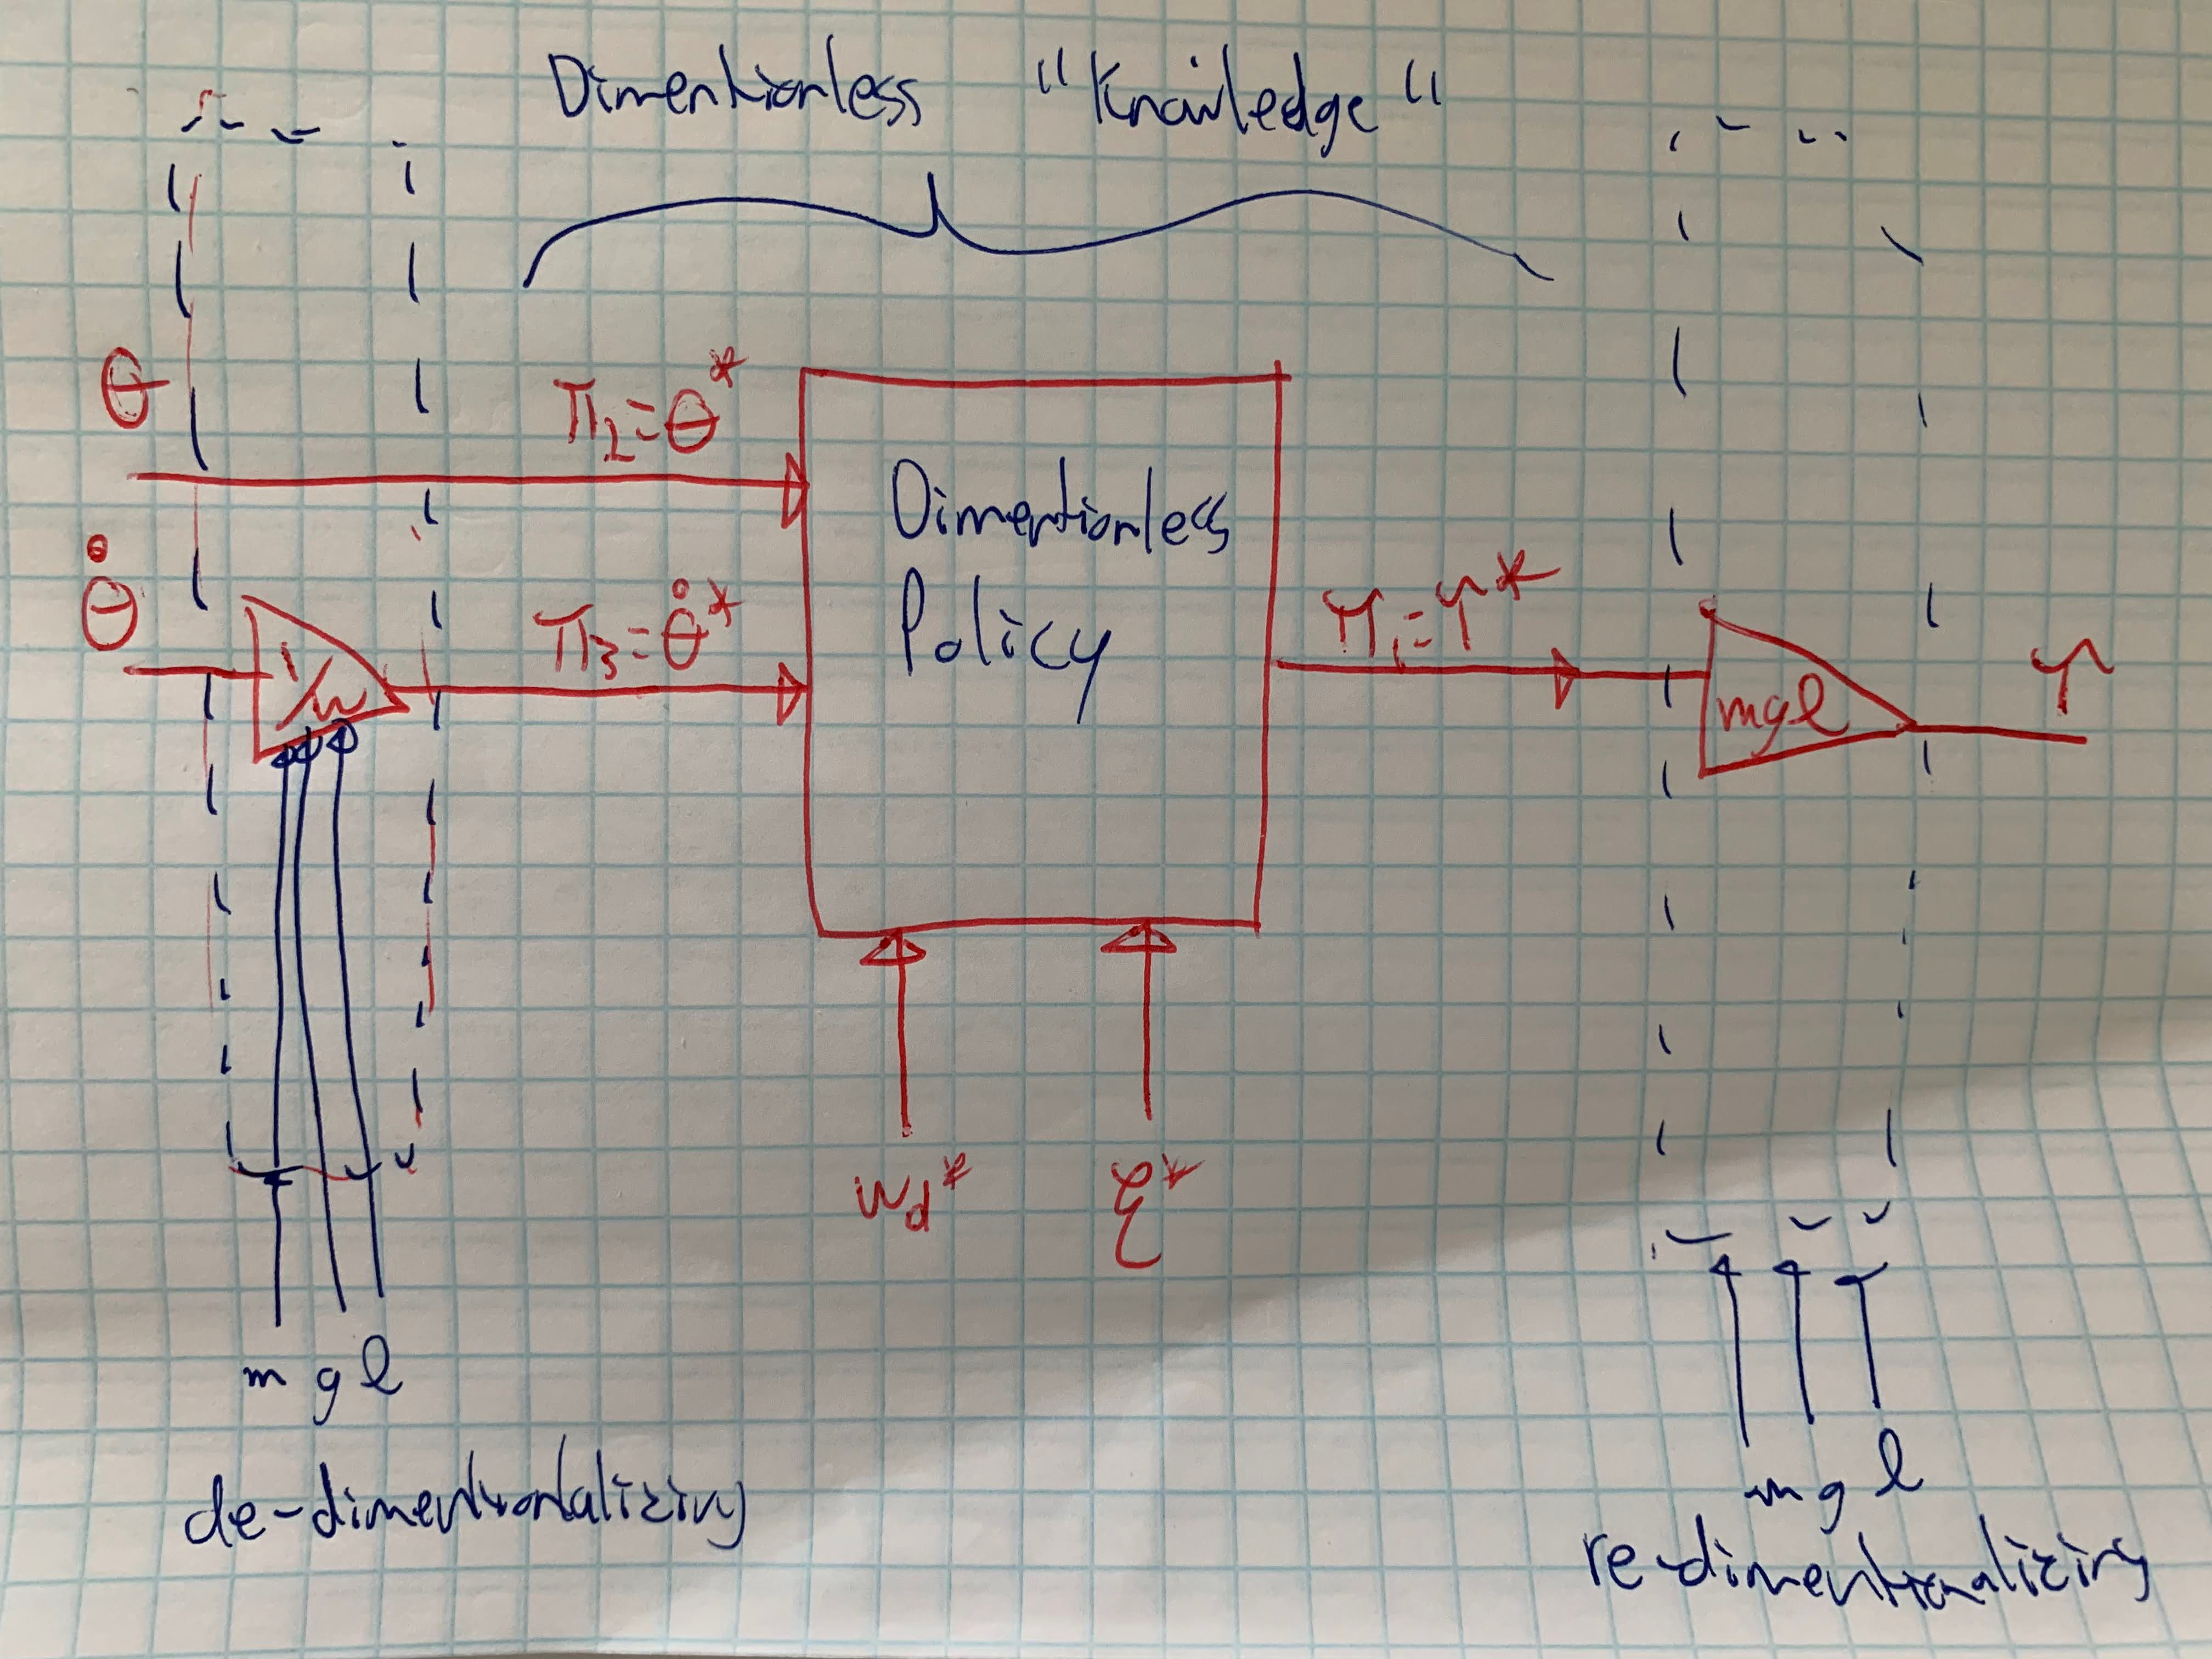
\includegraphics[width=0.99\linewidth]{fig/ct.JPG}
\caption{Dimentionless computed torque}\label{fig:ct}
\end{center}
\end{figure}
%%%%%%%%%%%%%%%%%%%%%%




\newpage
\subsection{Linear Quatratic Reglator (LQR) solution}


%%%%%%%%%%%%%%%%%%%%%%
\begin{equation}
\underbrace{\tau}_{\text{inputs}}
=
\pi \left(
\underbrace{ \theta, \dot{\theta} }_{\text{states}},
\underbrace{ m , g , l }_{\text{system parameters}},
\underbrace{ q }_{\text{task parameters}}
\right)
\end{equation}
%%%%%%%%%%%%%%%%%%%%%%

%%%%%%%%%%%%%%%%%%%%%%
\begin{equation}
\tau^*
=
\pi^* \left(
 \theta, \dot{\theta}^* ,
 q^* 
\right)
\end{equation}
%%%%%%%%%%%%%%%%%%%%%%


See alex screen shot 4 july 2023
%%%%%%%%%%%%%%%%%%%%%%
\begin{equation}
\tau = 
\left[
mgl \right] \theta
+
\left[
\sqrt{ (mgl)^2 + q^2} \right] \theta
+
\left[
\sqrt{ 2 ml^2)} \sqrt{mgl+ \sqrt{ (mgl)^2 + q^2}}
\right] \dot{\theta}^*
\end{equation}
%%%%%%%%%%%%%%%%%%%%%%

%%%%%%%%%%%%%%%%%%%%%%
\begin{equation}
\tau^* = 
\left[
1 + \sqrt{ 1 + (q^*)^2}
\right] \theta
+
\left[
\sqrt{2} \sqrt{ 1 + \sqrt{ 1 + (q^*)^2}}
\right] \dot{\theta}^*
\end{equation}
%%%%%%%%%%%%%%%%%%%%%%


\newpage
%%%%%%%%%%%%%%%%%%%%%%
\section{Numerical optimal policies}

%%%%%%%%%%%%%%%%%%%%%%%%%%%%%%%%%%%%%%%%%%%%
\begin{table}[htb]
   \centering % center the table
   \caption{Pendulum swing-up problems parameters} 
   \begin{tabular}{ p{2.0cm} p{0.8cm} p{0.8cm} p{0.8cm} p{0.8cm} p{0.8cm} }
   \hline \hline \noalign{\smallskip} \noalign{\smallskip} 
   %%%%%%%%%%%%%%%%%%%%%%
      & $m$ & $g$ & $l$ & $q$ & $\tau_{max}$ \\ \hline
   %%%%%%%%%%%%%%%%%%%%%
   %%%%%%%%%%%%%%%%%%%%%%
   \hline \hline \noalign{\smallskip} 
   \multicolumn{6}{c}{\textbf{Problems with $\tau_{max}^* = 0.5$ and $q^* = 0.1$} }\\ \noalign{\smallskip}  \hline\hline  \noalign{\smallskip} 
   %%%%%%%%%%%%%%%%%%%%%%
   Context no 1 : & 1.0 & 10.0 & 1.0 & 1.0 & 5.0 \\
   Context no 2 : & 1.0 & 10.0 & 2.0 & 2.0 & 10.0 \\
   Context no 3 : & 2.0 & 10.0 & 1.0 & 2.0 & 10.0 \\
   %%%%%%%%%%%%%%%%%%%%%
   \hline \hline \noalign{\smallskip} 
   \multicolumn{6}{c}{\textbf{Problems with $\tau_{max}^* = 1.0$ and $q^* = 0.05$} }\\ \noalign{\smallskip}  \hline\hline  \noalign{\smallskip} 
   %%%%%%%%%%%%%%%%%%%%%%
   Context no 4 : & 1.0 & 10.0 & 1.0 & 0.5 & 10.0 \\
   Context no 5 : & 1.0 & 10.0 & 2.0 & 1.0 & 20.0 \\
   Context no 6 : & 2.0 & 10.0 & 1.0 & 1.0 & 20.0 \\
   %%%%%%%%%%%%%%%%%%%%%
   \hline \hline \noalign{\smallskip} 
   \multicolumn{6}{c}{\textbf{Problems with $\tau_{max}^* = 1.0$ and $q^* = 10$} }\\ \noalign{\smallskip}  \hline\hline  \noalign{\smallskip} 
   %%%%%%%%%%%%%%%%%%%%%%
   Context no 7 : & 1.0 & 10.0 & 1.0 & 100.0 & 10.0 \\
   Context no 8 : & 1.0 & 10.0 & 2.0 & 200.0 & 20.0 \\
   Context no 9 : & 2.0 & 10.0 & 1.0 & 200.0 & 20.0 \\
   %%%%%%%%%%%%%%%%%%%%%
   \hline \hline
   \end{tabular}
\end{table}
%%%%%%%%%%%%%%%%%%%%%%%%%%%%%%%%%%%%%%%%%%%%

\subsection{Additionnal dimentionless parameters for the solver}

Using dynamic programming for solving the optimal policy numerically require setting additionnal parameter that define the domain. Altough those parameter should not affect the optimal policy far away from the boundaries, here a dimensionless version of those parameters was kept fixed in all the experiments:
%%%%%%%%%%%%%%%%%%%%%%
\begin{align}
\theta^*_{max} &= \theta_{max} = 2 \pi \\
\dot{\theta}^*_{max} &= \frac{ \dot{\theta}_{max} }{\omega} = 2 \\
t^*_{f} &= t_{f} \; \omega = 10 \times 2 \pi 
\end{align}
%%%%%%%%%%%%%%%%%%%%%%
$\theta_{max}$ is the range of angle for witch the optimal policy is solved, here set at one full revolution. $\dot{\theta}_{max}$ is the range of angular velocity for witch the optimal policy is solved, here the dimentionless ratio scaled with the natural frequency is set at 2. $t_{f}$ is the time horizon, here its associated dimentionless ratio is fixed to always corespond to 10 periods of the pendulum using the natural frequency.






\newpage

%%%%%%%%%%%%%%%%%%%%%%
\begin{equation}
\tau^*
=
\pi^* \left(
\theta, \dot{\theta}^*,
q^*=0.1 , \tau_{max}^* = 0.5
\right)
\end{equation}
%%%%%%%%%%%%%%%%%%%%%%

%%%%%%%%%%%%%%%%%%%%%%
\begin{figure}[H]
\begin{center}
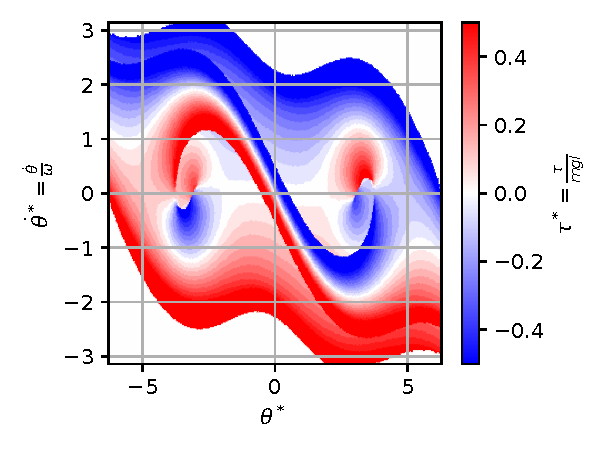
\includegraphics[width=0.99\linewidth]{fig/c1_dimpolicy.pdf}
\caption{Context no 1, 2 and 4 dimentionless optimal policy}\label{fig:c1_policy}
\end{center}
\end{figure}
%%%%%%%%%%%%%%%%%%%%%%

%%%%%%%%%%%%%%%%%%%%%%
\begin{equation}
\tau^*
=
\pi^* \left(
\theta, \dot{\theta}^*,
q^*=0.05 , \tau_{max}^* = 1.0
\right)
\end{equation}
%%%%%%%%%%%%%%%%%%%%%%

%%%%%%%%%%%%%%%%%%%%%%
\begin{figure}[H]
\begin{center}
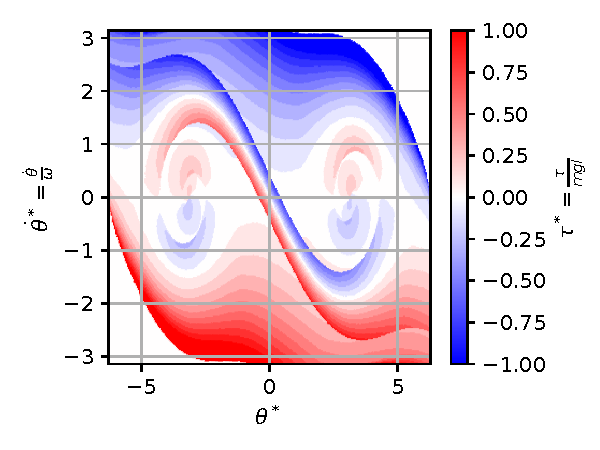
\includegraphics[width=0.99\linewidth]{fig/c4_dimpolicy.pdf}
\caption{Context no 4, 5 and 6 dimentionless optimal policy}\label{fig:c1_policy}
\end{center}
\end{figure}
%%%%%%%%%%%%%%%%%%%%%%

%%%%%%%%%%%%%%%%%%%%%%
\begin{equation}
\tau^*
=
\pi^* \left(
\theta, \dot{\theta}^*,
q^* = 10 , \tau_{max}^* = 1.0
\right)
\end{equation}
%%%%%%%%%%%%%%%%%%%%%%
%%%%%%%%%%%%%%%%%%%%%%
\begin{figure}[H]
\begin{center}
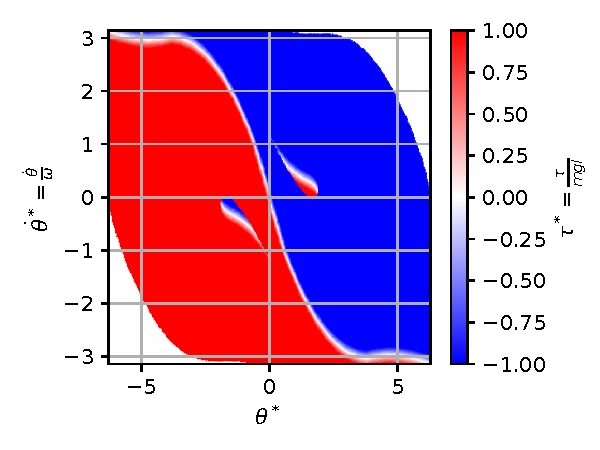
\includegraphics[width=0.99\linewidth]{fig/c7_dimpolicy.pdf}
\caption{Context no 7, 8 and 9 dimentionless optimal policy}\label{fig:c1_policy}
\end{center}
\end{figure}
%%%%%%%%%%%%%%%%%%%%%%












%  \begin{figure}[ht]
%     \centering
%     \vspace{-10pt}
%     \subfloat[Small vehicle \label{fig:a}]{\includegraphics[width=0.12\textwidth]{fig/a.jpg}}
%     \subfloat[Long vehicle \label{fig:b}]{\includegraphics[width=0.18\textwidth]{fig/b.jpg}}   
%     \subfloat[Large vehicle \label{fig:c}]{\includegraphics[width=0.16\textwidth]{fig/c.PNG}}
%     \caption{subfigures}
%     \label{fig:subfigures}
% \end{figure}











%%%%%%%%%%%%%%%%%%%%%%
\begin{figure}[p]
\begin{center}
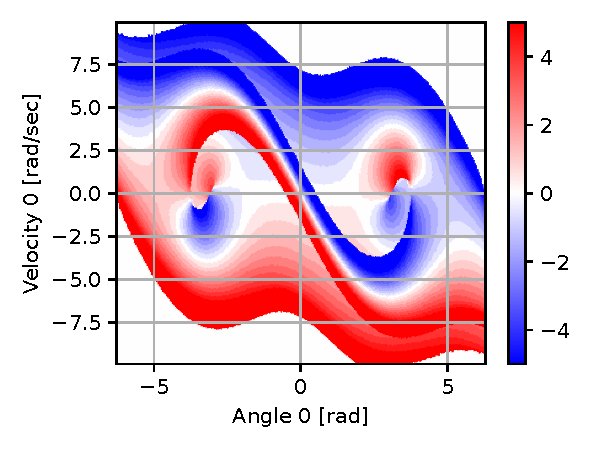
\includegraphics[width=0.99\linewidth]{fig/c1_policy.pdf}
\caption{Context no 1 optimal policy}\label{fig:c1_policy}
\end{center}
\end{figure}
%%%%%%%%%%%%%%%%%%%%%%


%%%%%%%%%%%%%%%%%%%%%%
\begin{figure}[p]
\begin{center}
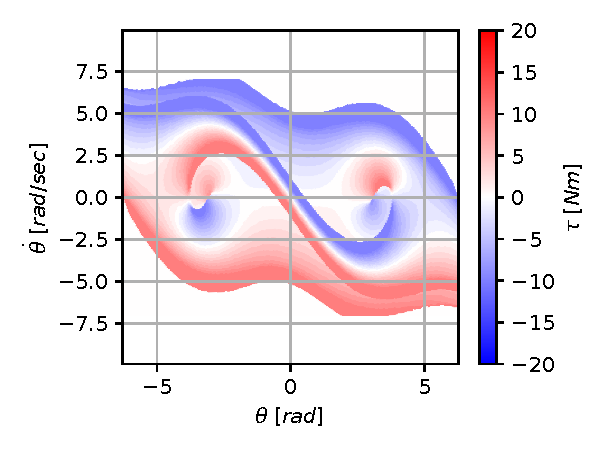
\includegraphics[width=0.99\linewidth]{fig/c2_policy.pdf}
\caption{Context no2 optimal policy}\label{fig:c1_policy}
\end{center}
\end{figure}
%%%%%%%%%%%%%%%%%%%%%%

%%%%%%%%%%%%%%%%%%%%%%
\begin{figure}[p]
\begin{center}
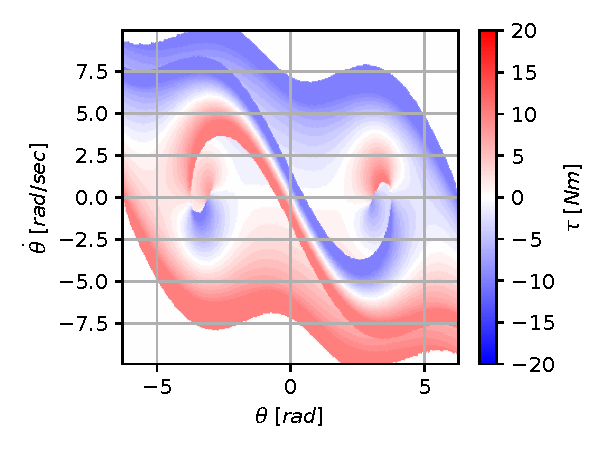
\includegraphics[width=0.99\linewidth]{fig/c3_policy.pdf}
\caption{Context no3 optimal policy}\label{fig:c1_policy}
\end{center}
\end{figure}
%%%%%%%%%%%%%%%%%%%%%%

\newpage
%%%%%%%%%%%%%%%%%%%%%%
\begin{figure}[p]
\begin{center}
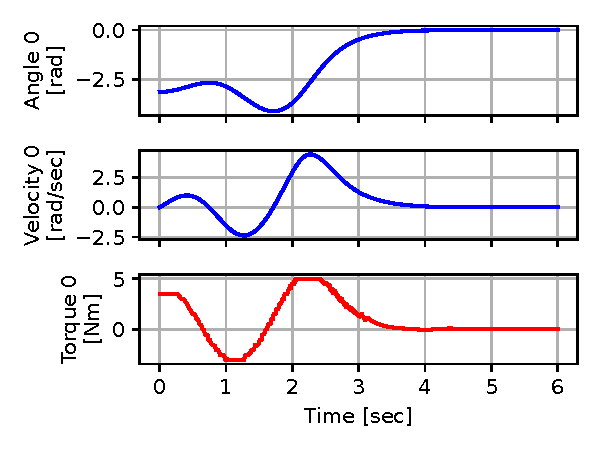
\includegraphics[width=0.99\linewidth]{fig/c1_traj.pdf}
\caption{Context no1 optimal trajectory from up-down position}\label{fig:c1_traj}
\end{center}
\end{figure}
%%%%%%%%%%%%%%%%%%%%%%


%%%%%%%%%%%%%%%%%%%%%%
\begin{figure}[p]
\begin{center}
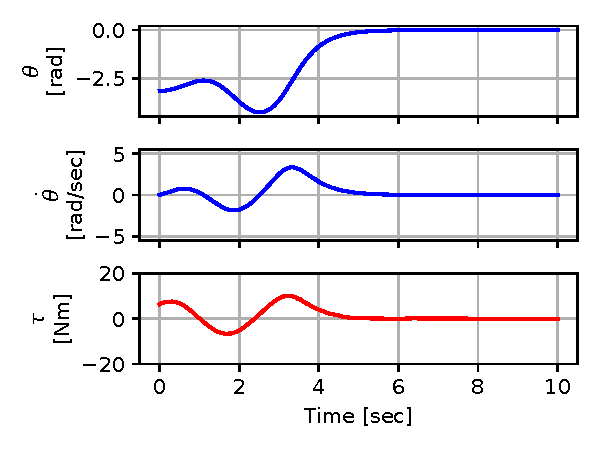
\includegraphics[width=0.99\linewidth]{fig/c2_traj.pdf}
\caption{Context no2 optimal trajectory from up-down position}\label{fig:c2_traj}
\end{center}
\end{figure}
%%%%%%%%%%%%%%%%%%%%%%

%%%%%%%%%%%%%%%%%%%%%%
\begin{figure}[p]
\begin{center}
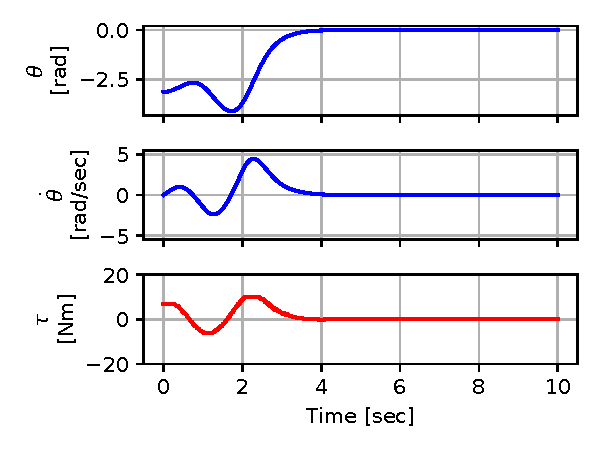
\includegraphics[width=0.99\linewidth]{fig/c3_traj.pdf}
\caption{Context no3 optimal trajectory from up-down position}\label{fig:c3_traj}
\end{center}
\end{figure}
%%%%%%%%%%%%%%%%%%%%%%


%%%%%%%%%%%%%%%%%%%%%%
\begin{figure}[p]
\begin{center}
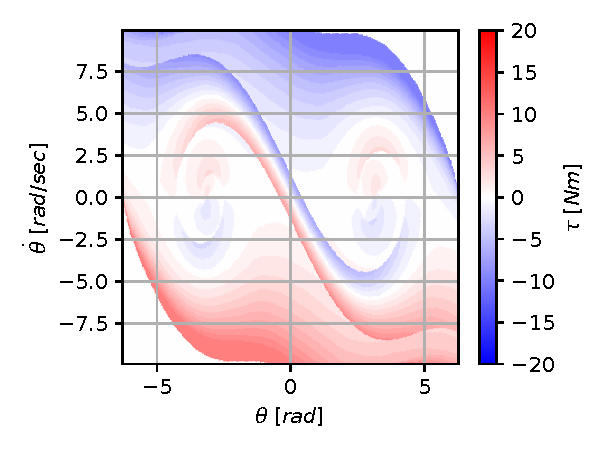
\includegraphics[width=0.99\linewidth]{fig/c4_policy.pdf}
\caption{Context no 4 optimal policy}\label{fig:c4_policy}
\end{center}
\end{figure}
%%%%%%%%%%%%%%%%%%%%%%


%%%%%%%%%%%%%%%%%%%%%%
\begin{figure}[p]
\begin{center}
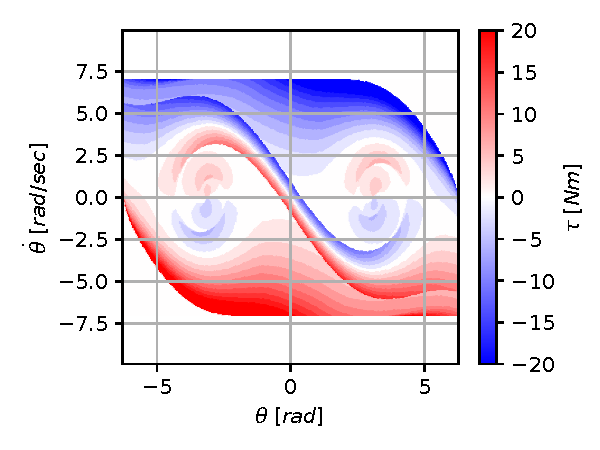
\includegraphics[width=0.99\linewidth]{fig/c5_policy.pdf}
\caption{Context no5 optimal policy}\label{fig:c5_policy}
\end{center}
\end{figure}
%%%%%%%%%%%%%%%%%%%%%%

%%%%%%%%%%%%%%%%%%%%%%
\begin{figure}[p]
\begin{center}
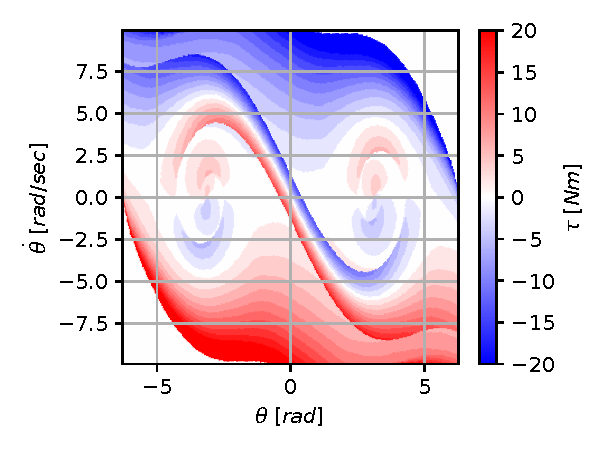
\includegraphics[width=0.99\linewidth]{fig/c6_policy.pdf}
\caption{Context no6 optimal policy}\label{fig:c6_policy}
\end{center}
\end{figure}
%%%%%%%%%%%%%%%%%%%%%%

\newpage
%%%%%%%%%%%%%%%%%%%%%%
\begin{figure}[p]
\begin{center}
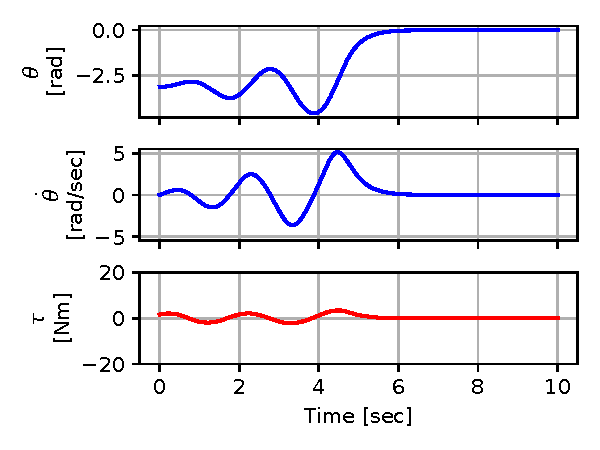
\includegraphics[width=0.99\linewidth]{fig/c4_traj.pdf}
\caption{Context no4 optimal trajectory from up-down position}\label{fig:c4_traj}
\end{center}
\end{figure}
%%%%%%%%%%%%%%%%%%%%%%


%%%%%%%%%%%%%%%%%%%%%%
\begin{figure}[p]
\begin{center}
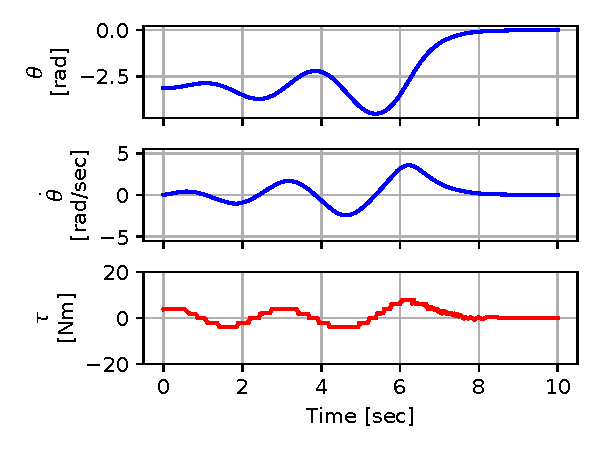
\includegraphics[width=0.99\linewidth]{fig/c5_traj.pdf}
\caption{Context no5 optimal trajectory from up-down position}\label{fig:c5_traj}
\end{center}
\end{figure}
%%%%%%%%%%%%%%%%%%%%%%

%%%%%%%%%%%%%%%%%%%%%%
\begin{figure}[p]
\begin{center}
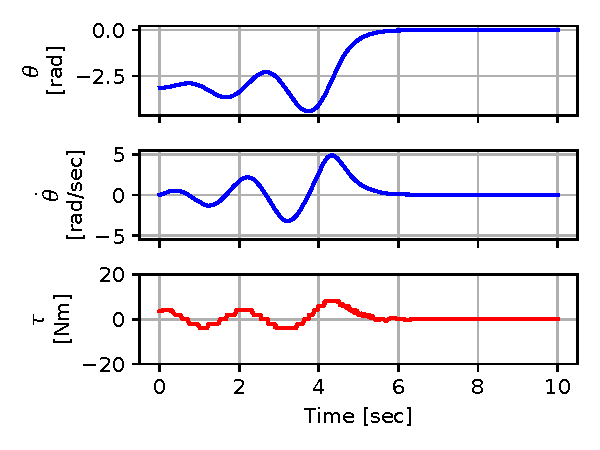
\includegraphics[width=0.99\linewidth]{fig/c6_traj.pdf}
\caption{Context no6 optimal trajectory from up-down position}\label{fig:c6_traj}
\end{center}
\end{figure}
%%%%%%%%%%%%%%%%%%%%%%


%%%%%%%%%%%%%%%%%%%%%%
\begin{figure}[p]
\begin{center}
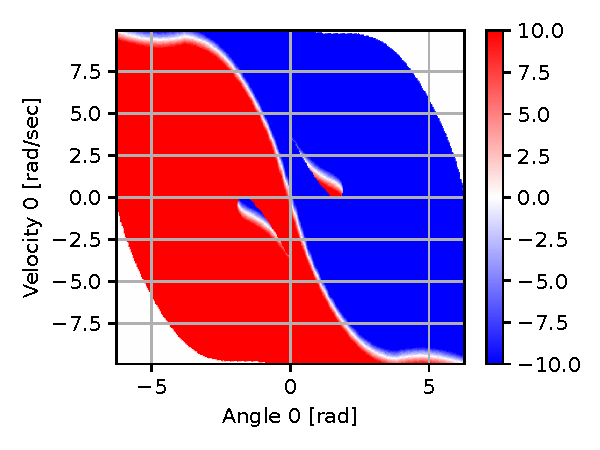
\includegraphics[width=0.99\linewidth]{fig/c7_policy.pdf}
\caption{Context no 7 optimal policy}\label{fig:c7_policy}
\end{center}
\end{figure}
%%%%%%%%%%%%%%%%%%%%%%


%%%%%%%%%%%%%%%%%%%%%%
\begin{figure}[p]
\begin{center}
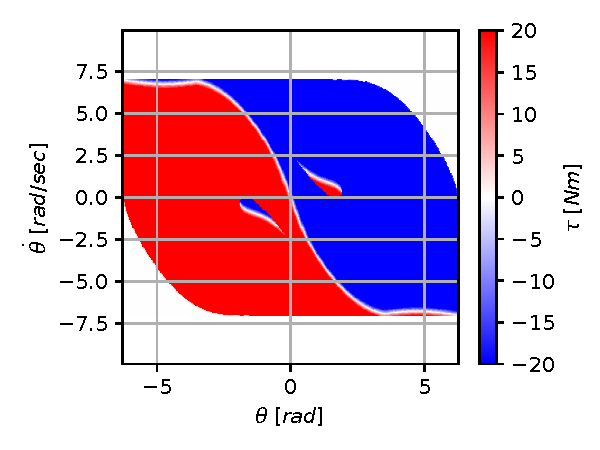
\includegraphics[width=0.99\linewidth]{fig/c8_policy.pdf}
\caption{Context no8 optimal policy}\label{fig:c8_policy}
\end{center}
\end{figure}
%%%%%%%%%%%%%%%%%%%%%%

%%%%%%%%%%%%%%%%%%%%%%
\begin{figure}[p]
\begin{center}
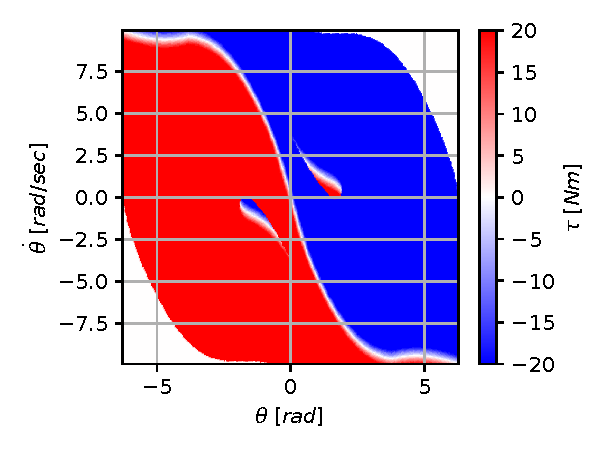
\includegraphics[width=0.99\linewidth]{fig/c9_policy.pdf}
\caption{Context no9 optimal policy}\label{fig:c9_policy}
\end{center}
\end{figure}
%%%%%%%%%%%%%%%%%%%%%%

\newpage
%%%%%%%%%%%%%%%%%%%%%%
\begin{figure}[p]
\begin{center}
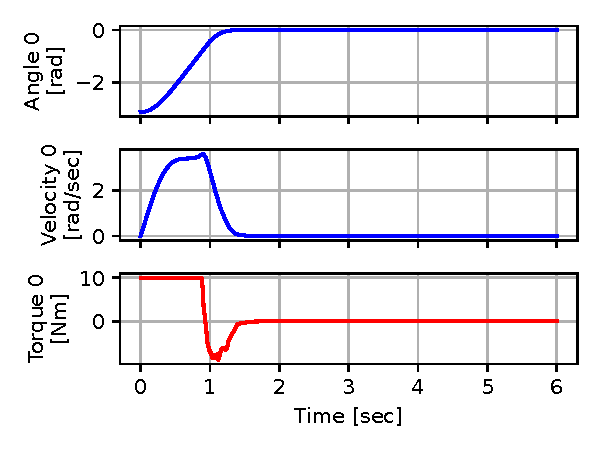
\includegraphics[width=0.99\linewidth]{fig/c7_traj.pdf}
\caption{Context no7 optimal trajectory from up-down position}\label{fig:c7_traj}
\end{center}
\end{figure}
%%%%%%%%%%%%%%%%%%%%%%


%%%%%%%%%%%%%%%%%%%%%%
\begin{figure}[p]
\begin{center}
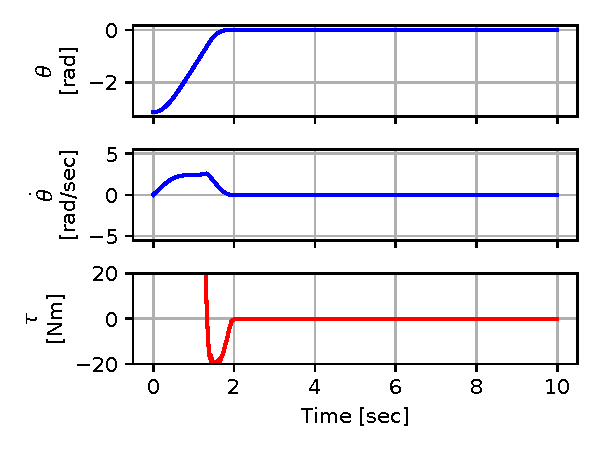
\includegraphics[width=0.99\linewidth]{fig/c8_traj.pdf}
\caption{Context no8 optimal trajectory from up-down position}\label{fig:c8_traj}
\end{center}
\end{figure}
%%%%%%%%%%%%%%%%%%%%%%

%%%%%%%%%%%%%%%%%%%%%%
\begin{figure}[p]
\begin{center}
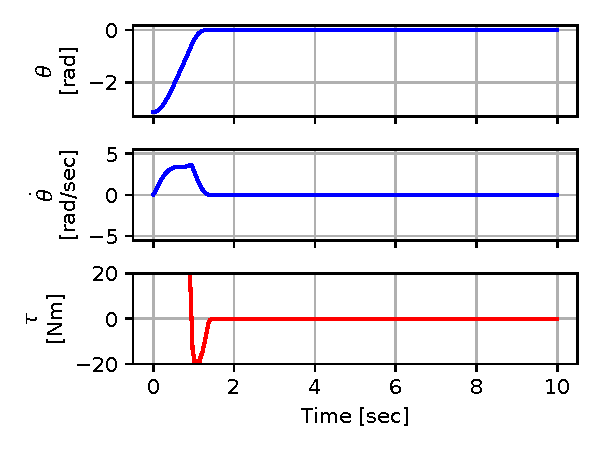
\includegraphics[width=0.99\linewidth]{fig/c9_traj.pdf}
\caption{Context no9 optimal trajectory from up-down position}\label{fig:c9_traj}
\end{center}
\end{figure}
%%%%%%%%%%%%%%%%%%%%%%



